\subsection{Transcriptomics data} \label{rnaSeq-data-sect}
The \emph{transcriptome} is the complete set of RNA molecules and their quantity, produced in a given cell or cell population at a given time. Measuring and analysing the trancriptome is essential for understanding major cellular processes, such as differentiation and carcinogenesis, and also for interpreting functional elements of the genome. 

The main approaches to deduce and quantify the transcriptome are based either on microarray hybridization, or on sequence-based techniques. \emph{Microarray hybridization} experiments \citep{Babu2004} were the method of choice until recently, but they had several limitations, including high background noise, limited dynamic range of detection, and reliance on good knowledge of an organism's genome. 

With the advent of NGS technology, \emph{RNA-Seq} (RNA sequencing) experiments \citep{Wang2009} are widely used for transcriptome profiling. The process for generating RNA-Seq data is simple and is shown in \emph{Fig. \ref{rnaSeq-pic}}. Initially some RNA fraction of interest is isolated for further analysis, \eg mRNA which mostly contains poly(A) at its tails. Then, the selected RNA is fragmented and reverse transcribed for the synthesis of cDNA libraries. Millions of reads are then obtained by sequencing the cDNA molecules using massively parallel sequencing technologies. The resulting reads are then aligned and mapped to a \emph{reference genome} (\ie transcriptome assembly), using alignment tools such as \emph{Bowtie} \citep{Langmead2009} and \emph{TopHat} \citep{Trapnell2009}. Finally, the number of reads that were mapped to specific genes are analysed to quantify gene expression \citep{Pepke2009}. Since we have non-negative read count data, a natural choice is to model the observations using a \emph{Poisson} distribution.
\begin{figure}[!ht]
\begin{center}
 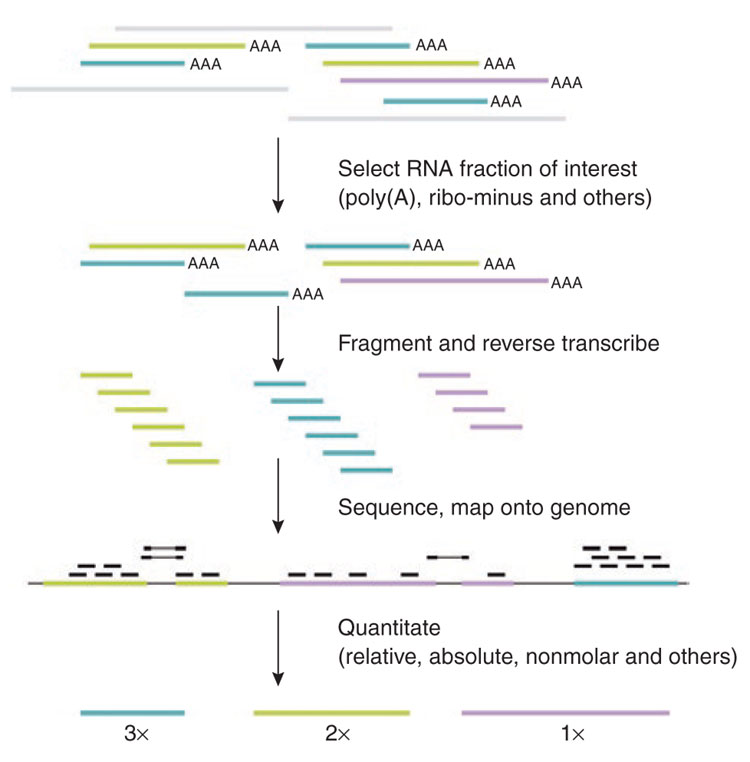
\includegraphics[scale = 0.37]{images/rna-seq}
\caption{\emph{Outline of RNA-Seq method. First, RNA is isolated, and then it is fragmented and reverse transcribed for synthesis of cDNA library. The cDNA is sequenced to produce millions of short reads and these reads are then aligned and mapped to a reference genome. Quantitative analysis of gene expression is based on the read counts \citep{Pepke2009}.}}
\label{rnaSeq-pic}
\end{center}
\end{figure}

A crucial step for RNA-Seq experiments is data normalization. Due to artifacts in the experiments, the data in different replicates or different biological conditions may not follow the same distribution, thus they cannot be directly compared. For example, read counts highly depend on the sequencing depth of the experiment, thus different samples might have different total number of reads, which may not be due to actual difference in gene expression. Also, longer transcripts will have in general more reads mapped to them compared to shorter transcripts of similar gene expression. Thus, transcript length normalization is required, and the most common choice is FPKM (Fragments Per Kilobase transcript per Million reads). \citet{Robinson2010} and \citet{Aleksic2014} provide an overview of different normalization methods needed for correctly analysing NGS experiments.
